\documentclass[10pt]{../usamts}

\realname{Juni Kim}
\username{junikimm}
\usamtsid{38002}
\usamtsyear{35}
\usamtsround{2}

\begin{document}

%%%%%%%%%%%%%%%%%%%%%%%%%%%%%%%%%%%%%
%%%%%%%%%%                 %%%%%%%%%%
%%%%%%%%%%    Problem 1    %%%%%%%%%%
%%%%%%%%%%                 %%%%%%%%%%
%%%%%%%%%%%%%%%%%%%%%%%%%%%%%%%%%%%%%
\begin{solution}
\begin{figure}[h!]
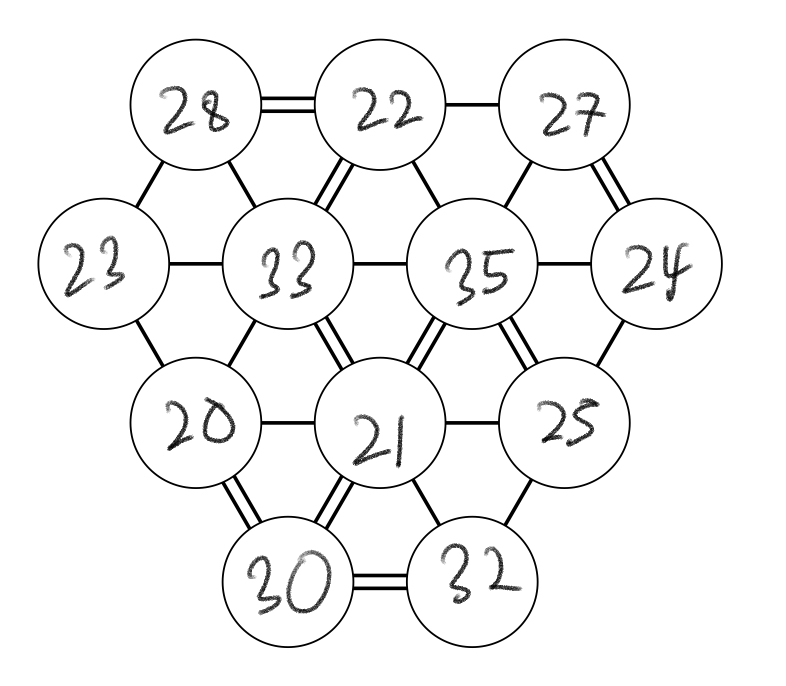
\includegraphics[width=5cm]{round2/solution1.jpeg}
\end{figure}
\end{solution}

%%%%%%%%%%%%%%%%%%%%%%%%%%%%%%%%%%%%%
%%%%%%%%%%                 %%%%%%%%%%
%%%%%%%%%%    Problem 2    %%%%%%%%%%
%%%%%%%%%%                 %%%%%%%%%%
%%%%%%%%%%%%%%%%%%%%%%%%%%%%%%%%%%%%%

\begin{solution}
We will just approach this by bashing. Let $a_n$ denote the number of six-digit codes possible when $n$ of the digits on the board have been smudged.
For our base case, $a_1 = 1$ because the only possible code is having all the digits be the same.
\begin{align*}
a_2 &= 2^6 - \binom{2}{1} \cdot a_1 = 62\\
a_3 &= 3^6 - \binom{3}{2} \cdot a_2 - \binom{3}{1} \cdot a_1 = 540\\
a_4 &= 4^6 - \binom{4}{3}\cdot a_3 - \binom{4}{2} \cdot a_2 - \binom{4}{1} \cdot a_1 = 1560\\
a_5 &= 5^6 - \binom{5}{4}\cdot a_4 - \binom{5}{3}\cdot a_3 - \binom{5}{2} \cdot a_2 - \binom{5}{1} \cdot a_1 = 1800\\
a_6 &= 6! = 720\\
\end{align*}

It is clear from this calculation that we get the most possible combinations when 5 of the digits have been smudged.

\end{solution}


%%%%%%%%%%%%%%%%%%%%%%%%%%%%%%%%%%%%%
%%%%%%%%%%                 %%%%%%%%%%
%%%%%%%%%%    Problem 3    %%%%%%%%%%
%%%%%%%%%%                 %%%%%%%%%%
%%%%%%%%%%%%%%%%%%%%%%%%%%%%%%%%%%%%%
\begin{solution}
Note that a set of three numbers is \textit{balanced} if and only if their sum is congruent to 0 mod 3.

Before we proceed, note that the rows will be 0-indexed from bottom to top. So, the top row will be row 9, while the bottom row will be row 0. We will also 0-index each hexagon on each row going from left to right. So, $a_{i,j}$ is the $i+1$th hexagon on the $j+1$th row from the bottom.

We start by independently filling in the bottom numbers such that they take the values $a_{0,0} \dots a_{0,9}$ going from left to right. We can freely choose each number because no three hexagons on the bottom row are mutually adjacent.

Now, we claim that the entire rest of the grid is determined by the bottom row. In particular, $$a_{i,j} \equiv (-1)^{i} \sum_{k=0}^{i} \binom{i}{k} a_{0,j+k} \mod 3$$

This is easy to see by induction. The base case, for row 0, is trivial. Now, note the \textit{balanced} condition implies that
\begin{align*}
    a_{i,j} &\equiv -\paren{a_{i-1,j}+a_{i-1,j+1}} \mod 3\\
            &= (-1)^{i} \paren{\sum_{k=0}^{i-1} \binom{i-1}{k} a_{0,j+k} + \sum_{k=0}^{i-1} \binom{i-1}{k} a_{0,j+1+k}}\\
            &= (-1)^{i}\paren{a_{0,j} + a_{0,i+j} + \sum_{k=0}^{i-2} \paren{\binom{i-1}{k} + \binom{i-1}{k+1}} a_{0,j+k+1} }\\
            &= (-1)^{i}\paren{a_{0,j} + a_{0,i+j} + \sum_{k=1}^{i-1} \binom{i}{k} a_{0,j+k} } \tag{hockey stick}\\
            &= (-1)^{i} \sum_{k=0}^{i} \binom{i}{k} a_{0,j+k}\\
\end{align*}

Note that
$$\binom{9}{0} = \binom{9}{9} = 1$$
$$\binom{9}{1} = \binom{9}{8} = 9, 3\,|\,9$$
$$\binom{9}{2} = \binom{9}{7} = 36, 3\,|\,36$$
$$\binom{9}{3} = \binom{9}{6} = 84, 3\,|\,84$$
$$\binom{9}{4} = \binom{9}{5} = 126, 3\,|\,126$$

So it is clear that
\begin{align*}
    a_{9,0} &\equiv -\paren{\sum_{k=0}^{9} \binom{9}{k} a_{0,k}} \mod 3\\
    &\equiv -\paren{a_{0,0} + a_{0,9}} \mod 3\\
\end{align*}

So, $a_{0,0} + a_{0,9} + a_{9,0} \equiv 0 \mod 3$, meaning they are balanced.

\end{solution}


%%%%%%%%%%%%%%%%%%%%%%%%%%%%%%%%%%%%%
%%%%%%%%%%                 %%%%%%%%%%
%%%%%%%%%%    Problem 4    %%%%%%%%%%
%%%%%%%%%%                 %%%%%%%%%%
%%%%%%%%%%%%%%%%%%%%%%%%%%%%%%%%%%%%%
\begin{solution}
\begin{figure}
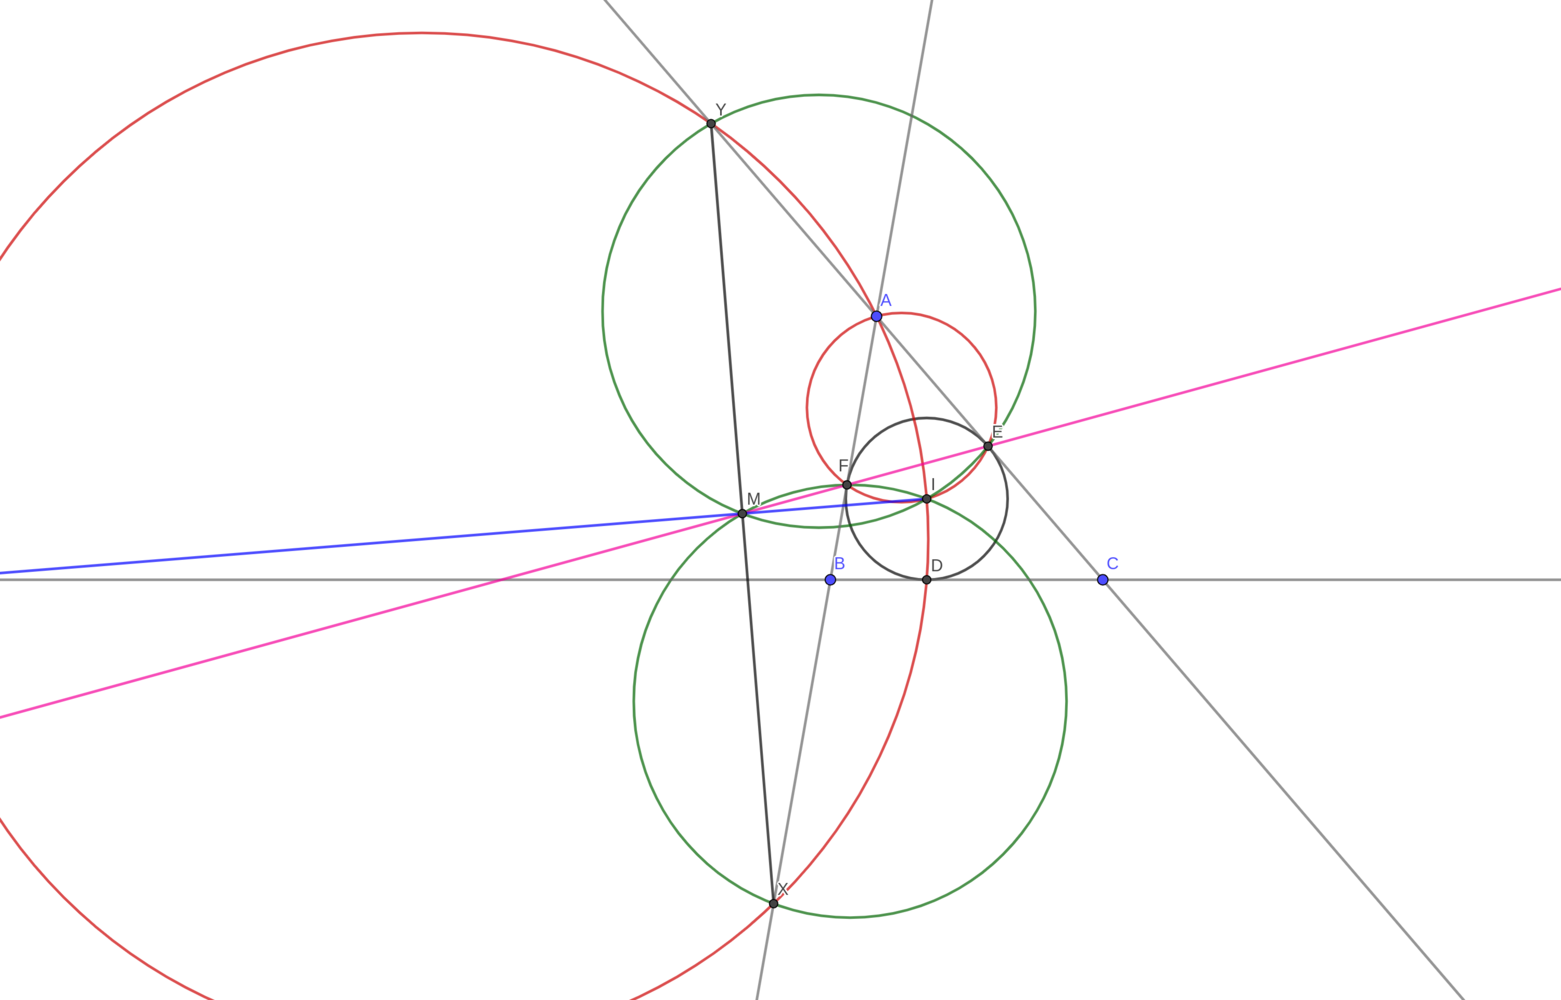
\includegraphics[width=12cm]{round2/p4diagram.png}
\caption{The Diagram}
\end{figure}

Note that $AFIE$ is obviously a cyclic quadrilateral. We therefore know that there is a spiral similarity that sends $\triangle FIE$ to $\triangle XIY$. Since $\triangle FIE$ is an isosceles triangle, so is $XIY$. Therefore, the midpoint of $XY$, which we denote $M$, is also the foot of the perpendicular from $I$ to $XY$. Since $\angle IEY = 90$ and $\angle IFX = 90$, It follows that $IEMY$ and $IFMX$ are cyclic quadrilaterals. Now, note that $\angle MFI = 180 - \angle MXI = 180 - \angle YXI = 180 - \angle EFI$ by the spiral similarity from before. So, $M,E,F$ are collinear and we are done.
\end{solution}

%%%%%%%%%%%%%%%%%%%%%%%%%%%%%%%%%%%%%
%%%%%%%%%%                 %%%%%%%%%%
%%%%%%%%%%    Problem 5    %%%%%%%%%%
%%%%%%%%%%                 %%%%%%%%%%
%%%%%%%%%%%%%%%%%%%%%%%%%%%%%%%%%%%%%
\begin{solution}
What a painful construction problem...

The answer is all $n,m$ such that $n+m \equiv 1 \mod 4$ or $n \equiv m \mod 4$.

We first prove that this condition must hold. Note that the sum of the x and y coordinates must be congruent to $\sum_{x=1}^{m+n-1} \sum_{y=1}^{m+n-1} 1 \equiv 0 \mod 2$. Now, the sum of all $x+y$ mod 2 is congruent to $\frac{1}{2}\paren{m+n-1}\paren{3m+n}$. This means that $(m+n-1)(n-m)$ must be congruent to 0 mod 4. Since $(m+n-1)$ and $(n-m)$ always differ in parity, either $n-m \equiv 0 \mod 4$ or $m + n - 1 \equiv 0 \mod 4$.

Now, we present highly generalizable constructions for all six cases of $m,n$ modulo 4.

\begin{figure}[h!]
    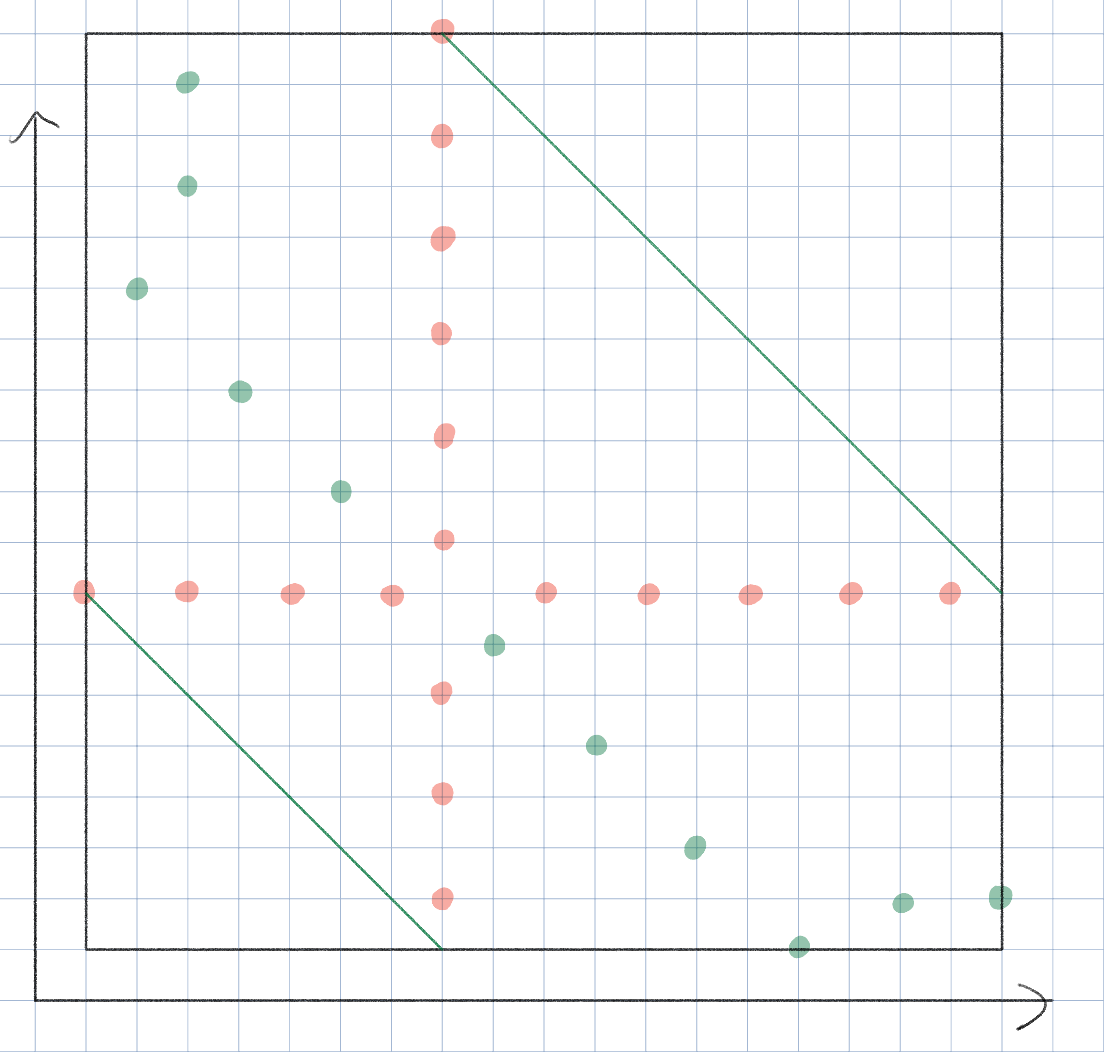
\includegraphics[width=10cm]{round2/p5construct/construct_8_12.png}
    \caption{Construction for when n and m are both congruent to 0 mod 4}
\end{figure}
\begin{figure}[h!]
    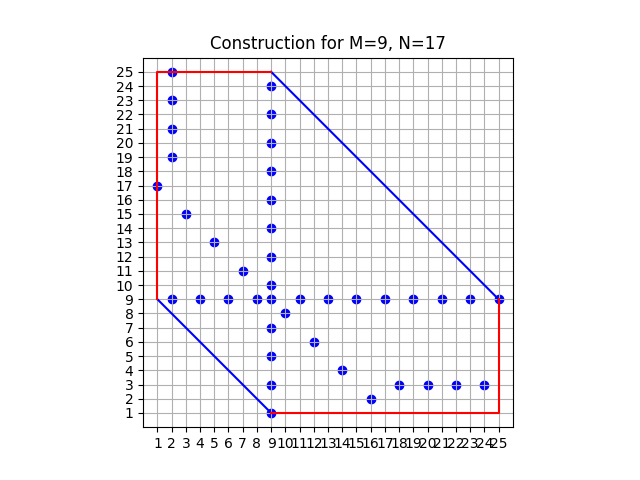
\includegraphics[width=10cm]{round2/p5construct/construct_9_17.png}
    \caption{Construction for when n and m are both congruent to 1 mod 4}
\end{figure}
\begin{figure}[h!]
    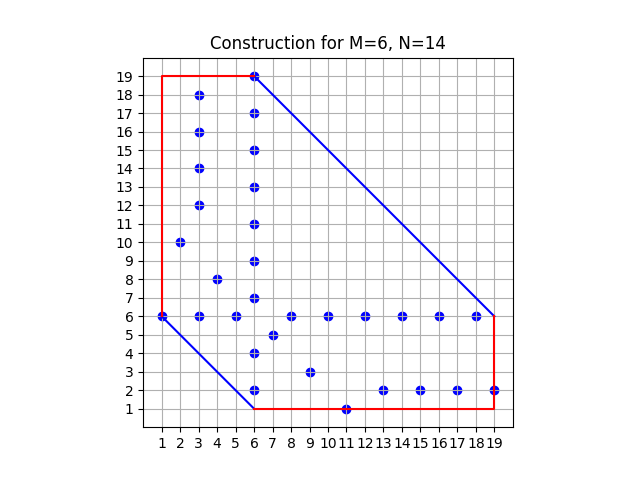
\includegraphics[width=10cm]{round2/p5construct/construct_6_14.png}
    \caption{Construction for when n and m are both congruent to 2 mod 4}
\end{figure}
\begin{figure}[h!]
    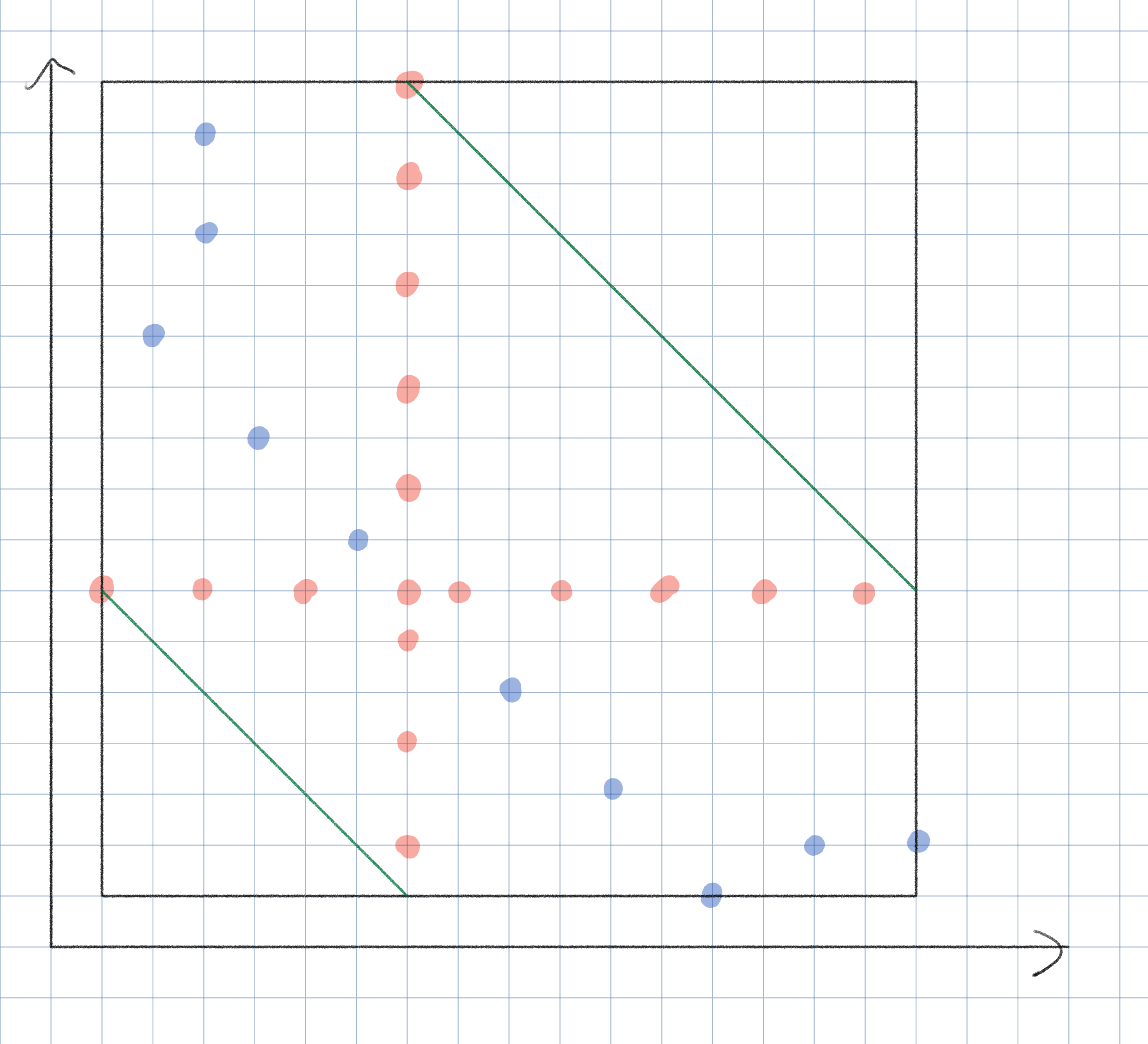
\includegraphics[width=10cm]{round2/p5construct/construct_7_11.png}
    \caption{Construction for when n and m are both congruent to 3 mod 4}
\end{figure}

\begin{figure}[h!]
    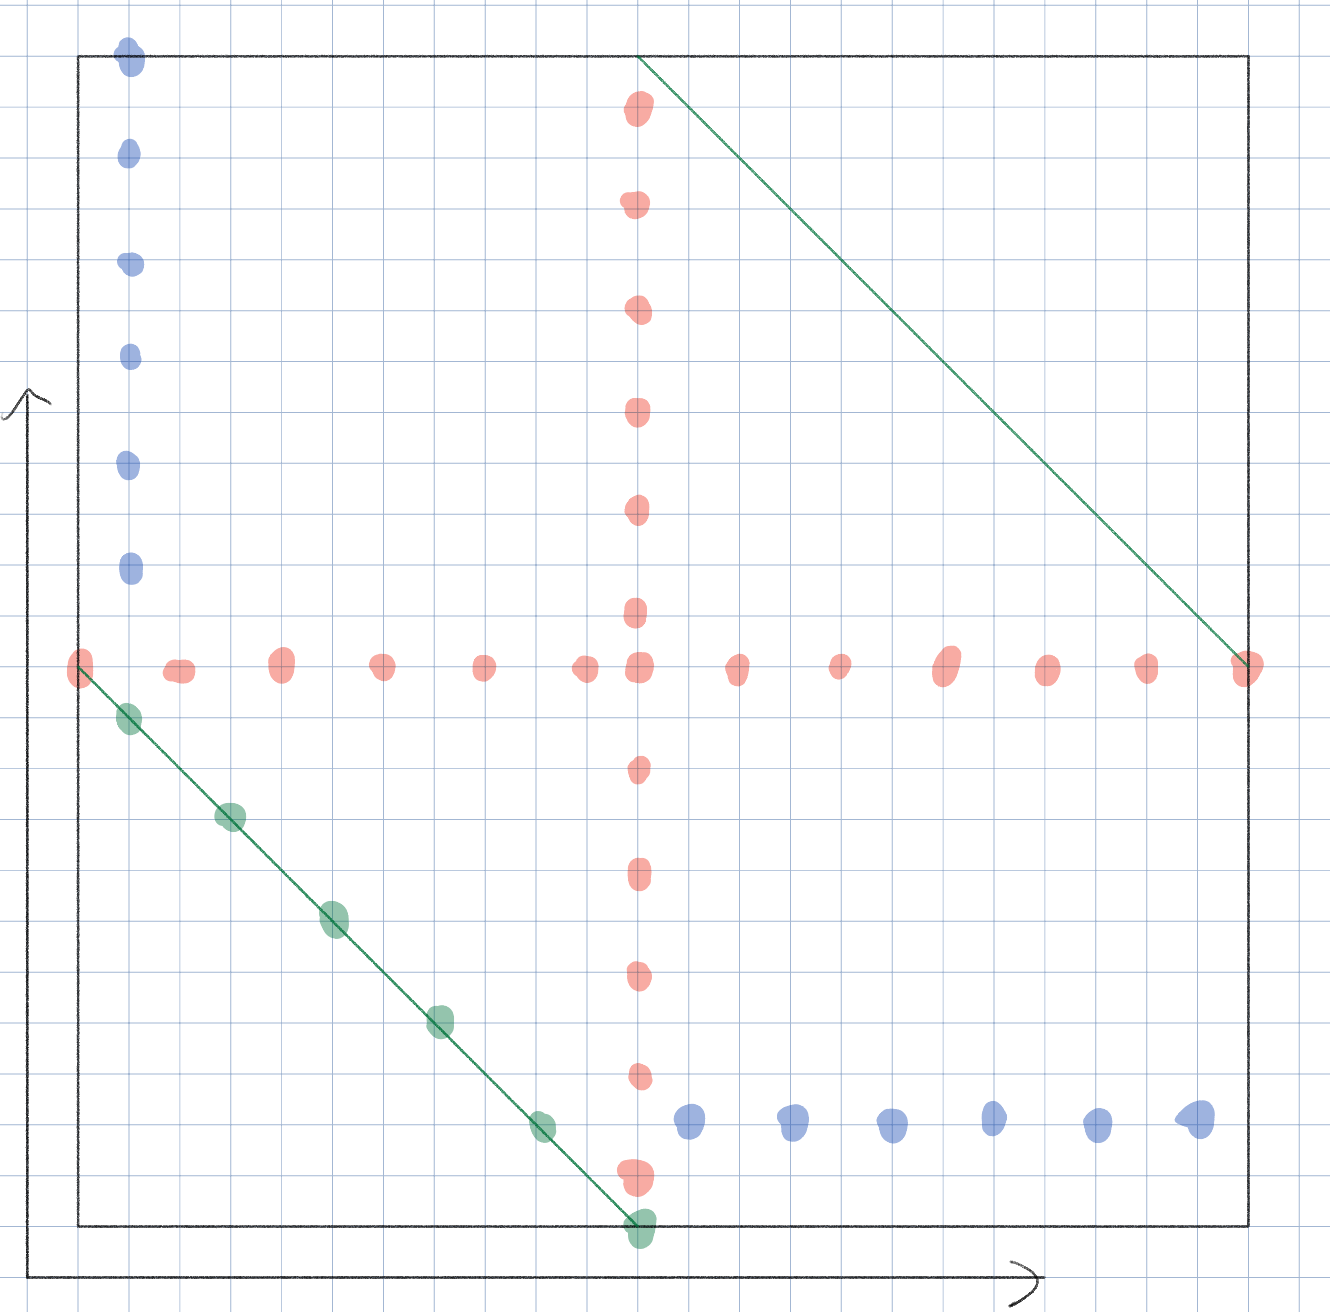
\includegraphics[width=10cm]{round2/p5construct/construct_12_13.png}
    \caption{Construction for when m is congruent to 0 mod 4 and n is congruent to 1 mod 4. If the reverse is true, just flip the construction.}
\end{figure}
\begin{figure}[h!]
    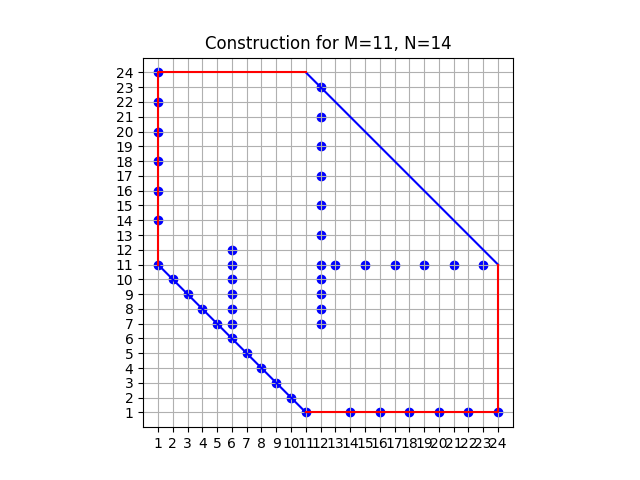
\includegraphics[width=10cm]{round2/p5construct/construct_11_14.png}
    \caption{Construction for when m is congruent to 3 mod 4 and n is congruent to 2 mod 4. If the reverse is true, just flip the construction.}
\end{figure}

\end{solution}

\end{document}